\documentclass[a4paper,10pt]{memoir}
\usepackage[italian]{babel}
\usepackage{wrapfig}
\usepackage[pdftex]{graphicx}
\usepackage{graphviz}

% import package
\usepackage{FrontespizioSapienza}

% declare info
\FSSTitolo{Ottimizzazione delle risorse nell'uso di servizi in background in SeismoCloud per Android}
\FSSFacolta{Facoltà di Ingegneria dell'Informazione, Informatica e Statistica}
\FSSCorso{Informatica}

\FSSCandidato{Enrico Bassetti}
\FSSMatricola{1401568}
\FSSRelatore{Emanuele Panizzi}
\FSSCorrelatore{}
\FSSAnnoAccademico{2016/2017}


\begin{document}
  
  
\frontmatter


% print title
\maketitle
\cleardoublepage

% rest of the document
\begin{abstract}
	\thispagestyle{plain}
	Sommario della tesi.
\end{abstract}
\cleardoublepage

\tableofcontents
\cleardoublepage

\mainmatter

\renewcommand\chapterheadstart{}
\renewcommand\printchaptername{}
\renewcommand\chapternamenum{}
\renewcommand\printchapternum{}
\renewcommand\afterchapternum{}
\renewcommand\printchaptertitle[1]{\chaptitlefont \thechapter. \space #1}

%\setlength{\intextsep}{1pt}%

\chapter{Introduzione}

\section{I terremoti e la loro origine}


\begin{wrapfigure}{r}{0.30\textwidth}
\label{fig:litosfera}
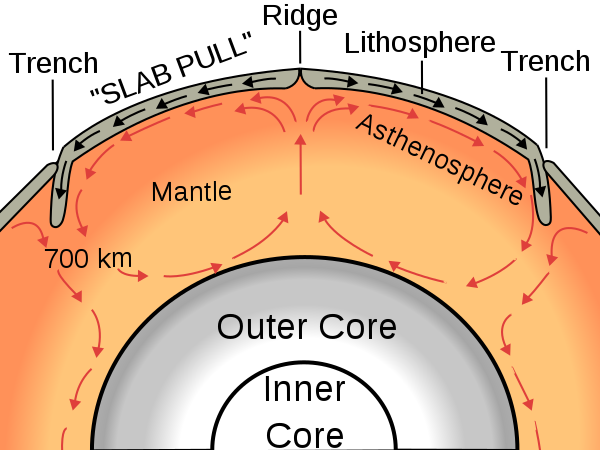
\includegraphics[width=0.30\textwidth]{introduzione/oceanic_spreading}
\end{wrapfigure}

La Terra è formata, nei primi 200 km di bordo esterno, da una zona chiamata \textit{litosfera}, di cui fa parte la \textit{crosta terrestre} con le terre emerse ed i fondali marini/oceanici. La \textit{litosfera} è divisa in parti, chiamate \textbf{placche tettoniche}, che "gallegiano" sul \textit{mantello superiore}. Queste placche sono continuamente spinte in direzioni diverse da \textit{moti convettivi} generati dalla temperatura elevata del nucleo. La zona di confine di queste placche viene chiamata \textbf{faglia}, e presenta diverse caratteristiche a seconda delle direzioni delle placche: se due placche si avvicinano, una delle due placche verrà immersa nel mantello sotto l'altra (\textit{subduzione}); se due placche si allontanano, una nuova parte della litosfera viene generata dalla roccia fusa proveniente dal mantello; infine, se due placche si muovo nella stessa direzione ma in senso opposto, siamo in presenza di \textit{margini di scorrimento}.

\begin{wrapfigure}[12]{r}{0.30\textwidth}
\label{fig:mappafaglie}
\caption{Mappa delle faglie italiane attive}
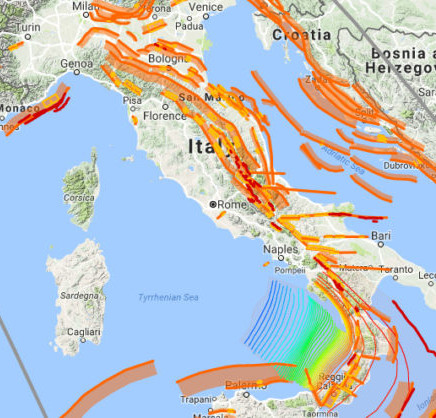
\includegraphics[width=0.30\textwidth]{introduzione/mappa_faglie_italiane2}
\end{wrapfigure}

Il movimento delle placche nei margini, tuttavia, non è libero da attrito: a seconda del materiale, della profondità e della conformazione della roccia presente nella faglia, la faglia stessa tende ad \textbf{opporsi} al movimento delle placche, accumulando energia da attrito, la quale viene rilasciata repentinamente, al superamento della massima forza d'attrito, come energia meccanica (le cosiddette \textit{onde sismiche}) generando un \textit{terremoto} (o sisma).

\section{Analisi e misura dei terremoti}

Per misurare l'energia sprigionata da un evento sismico, individuare il punto di origine (epicentro/ipocentro) e altre caratteristiche dell'onda si utilizzano i \textbf{sismometri}, apparati dotati di accelerometri molto precisi, filtri e amplificatori in grado di rilevare l'accelerazione sulle tre componenti (X-Y-Z) e produrre un \textit{sismogramma} (Figura \ref{fig:sismogramma}).

\begin{figure}[p]
\label{fig:retesensori}
\caption{La rete IV - Italian Seismic Network}
\centering
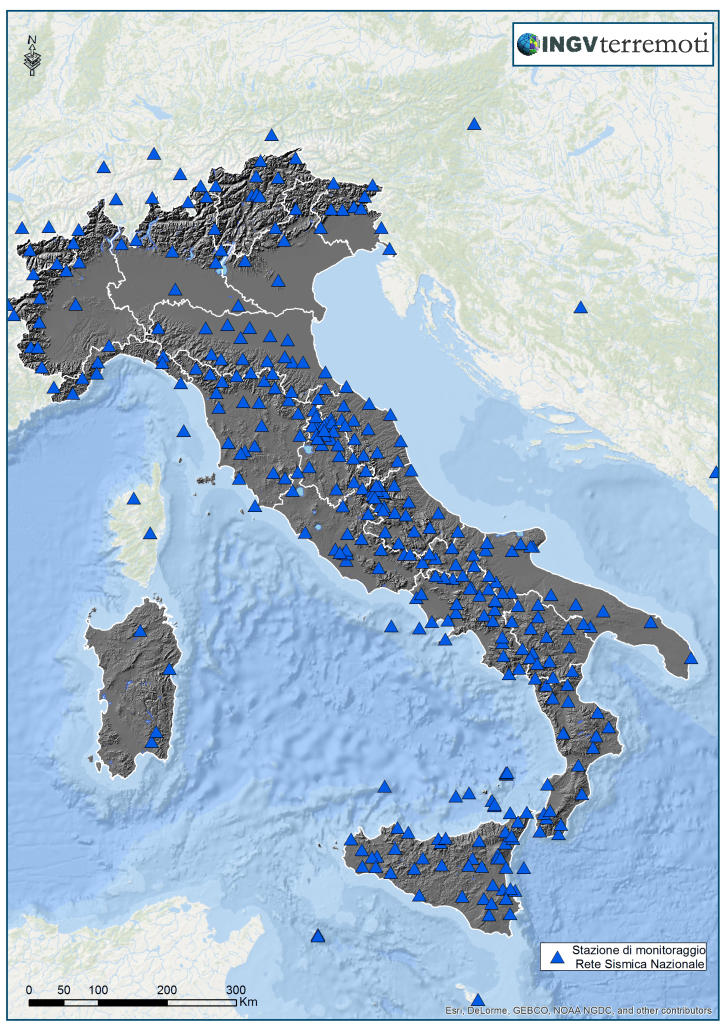
\includegraphics[width=10cm]{introduzione/rete_ingv}
\end{figure}

\begin{figure}[ht]
\label{fig:sismogramma}
\caption{Esempio di sismogramma}
\centering
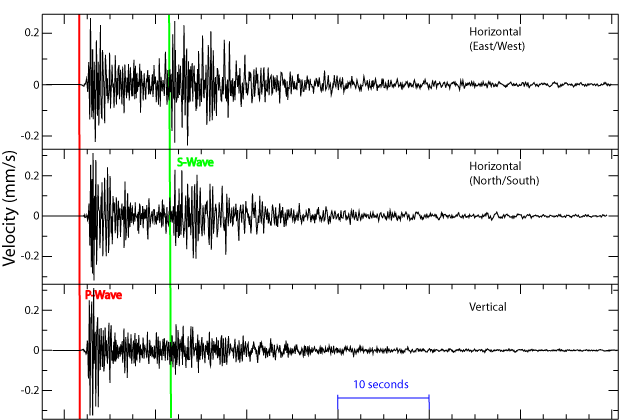
\includegraphics[width=10cm]{introduzione/seismogram}
\end{figure}

Attualmente nel mondo sono presenti diverse reti di rilevamento. Per l'Italia INGV riceve le informazioni da 27 reti sismiche (compresa la rete principale italiana \textit{IV - Italian Seismic Network}) per un totale di più di 800 sismometri (gran parte sul territorio nazionale, alcuni su paesi confinanti).

L'energia sprigionata viene misurata in \textbf{magnitudo} su una scala di valutazione chiamata \textbf{Richter}, mentre gli eventuali danni provocati vengono espressi in \textit{intensità del terremoto} tramite valori della scala \textbf{Mercalli-Cancani-Sieberg}, o MCS \footnote{Le due scale non hanno un legame diretto: un terremoto di piccola magnitudo può fare molti danni in alcune situazioni (e quindi essere di elevata intensità MCS); viceversa un terremoto di magnitudo molto elevata può avere intensità molto bassa in altre situazioni.}.

Infine possiamo distinguere il punto di origine del terremoto sotto la superficie, chiamato \textbf{epicentro}, e la proiezione di questo punto sulla superficie terrestre, chiamato \textbf{ipocentro} \footnote{Stein, Seth; Wysession, Michael (2009). An Introduction to Seismology, Earthquakes, and Earth Structure. John Wiley \& Sons. ISBN 978-1444311310}.

\begin{figure}[ht]
\label{fig:epiipo}
\caption{Epicentro, ipocentro (o focus) e faglia (\textit{fault plane})}
\centering
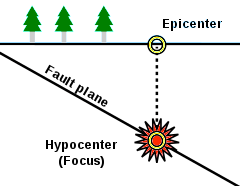
\includegraphics[scale=0.5]{introduzione/epicenter_diagram}
\end{figure}


\section{Prevedere o arginare i terremoti}

L'Italia è sottoposta, ogni giorno, ad un numero di terremoti nell'ordine del \textbf{centinaio di scosse}\footnote{Dati provenienti dal Centro Nazionale Terremoti: http://cnt.rm.ingv.it/}. Quasi tutti questi sismi sono classificati come \textit{microterremoti} (di magnitudo $<$ 2), poiché sono talmente deboli da essere percepibili solo dagli strumenti. Tuttavia, essendo l'Italia zona di confine tra la placca Europea e la placca Africana (con quest'ultima che si muove verso il Nord), la quantità di energia accumulata dalle faglie può generare terremoti in grado di infliggere ingenti danni.

Come in tutte le calamità naturali (e non), abbiamo diversi ambiti da considerare:
\begin{itemize}
\item la \textbf{prevenzione}, ovvero l'attuazione delle politiche in grado di minimizzare la probabilità che un evento accada e minimizzare il rischio all'accadere dell'evento
\item la \textbf{previsione}, ovvero l'utilizzo di tecniche e tecnologie che permettono di indicare \textit{quando un evento accadrà} (con una certa affidabilità)
\item la \textbf{gestione dell'emergenza} e del post-emergenza, ovvero delle azioni da mettere in campo durante e dopo il presentarsi di una calamità
\end{itemize}

Nella fattispecie dei terremoti, la \textbf{previsione} è tutt'ora materiale di studio da parte del mondo scientifico poiché risulta impossibile\footnote{Uyeda, Seiya; Nagao, Toshiyasu; Kamogawa, Masashi (2009-05-29), "Short-term earthquake prediction: Current status of seismo-electromagnetics", Tectonophysics, 470 (3–4): 205–213} prevedere, allo stato attuale, quando e dove accadrà il prossimo sisma \footnote{Alessandro Amato (2016). Sotto i nostri piedi. Codice edizioni, Torino. ISBN 978-8875785727}. Nel tempo, tuttavia, i vari dati raccolti riguardo ai terremoti hanno permesso di costruire delle mappe di pericolosità sismica\footnote{Pubblicate per la prima volta nel 2004 e poi aggiornate man mano: http://zonesismiche.mi.ingv.it/}, le quali indicano zone con maggiore probabilità di terremoti importanti, andando ad integrare le azioni di informazione e di formazione che fanno parte della \textbf{prevenzione}.

\begin{wrapfigure}[12]{r}{0.25\textwidth}
\centering
\label{fig:timelinecom}
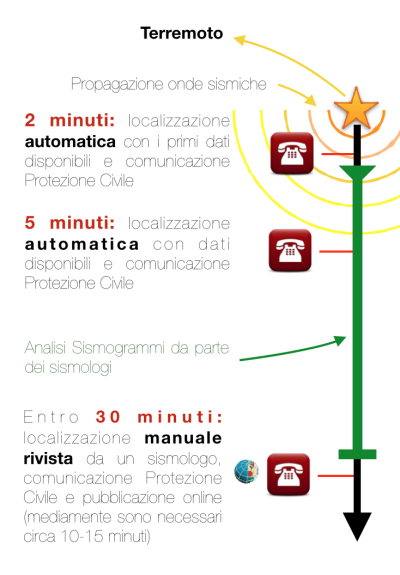
\includegraphics[width=0.25\textwidth]{introduzione/tempi_comunicazioni}
\end{wrapfigure}

Nella gestione dell'emergenza possiamo riportare quello che avviene allo stato attuale all'accadere di un terremoto, rilevato (per l'Italia) dalla rete di sismometri di INGV: nel momento in cui un sisma viene percepito da un numero congruo di stazioni di rilevamento, il sistema effettua verifiche e calcoli e, \textbf{entro due minuti}, è in grado di fornire una prima stima della magnitudo, dell'epicentro e della profondità (dati che poi vengono comunicati alla Protezione Civile). Successivamente, \textbf{entro 5 minuti} dal sisma, tutte le stazioni di rilevamento sono utilizzate per individuare le caratteristiche del terremoto in modo più preciso. Infine, \textbf{entro 30 minuti}, una verifica manuale da parte dei tecnici e ingegneri di INGV permette di avere il dato definitivo che viene di nuovo comunicato alla Protezione Civile e al pubblico \footnote{La pubblicazione avviene sul sito del Centro Nazionale Terremoti http://cnt.rm.ingv.it/ oppure tramite le pagine ufficiali sui principali Social Network}.

\section{Il progetto SeismoCloud}

Il progetto SeismoCloud nasce dalla collaborazione dall'\textbf{Università degli Studi di Roma "La Sapienza"} e l'\textbf{Istituto Nazionale di Geofisica e Vulcanologia}. L'obiettivo di questo progetto è quello di implementare un sistema di \textbf{early warning} in \textit{crowdsourcing}\footnote{Un sistema si dice in \textit{crowdsourcing} quando i dati per il suo funzionamento vengono forniti dagli stessi utenti} per i terremoti, in grado di inserirsi nel \textit{gap} presente dal momento in cui il terremoto accade, al momento in cui INGV è in grado di individuarlo. Lo scopo del sistema quindi è di individuare i terremoti \textit{in tempo reale}, alla loro apparizione nell'ipocentro, ed \textbf{anticipare} l'onda sismica (che viaggia, mediamente, ad una velocità di 5 km/s) avvertendo la popolazione nel raggio di azione del terremoto (questo sistema è chiamato, appunto \textit{early warning}).

Già da un decennio alcuni luoghi più sensibili al terremoto si stanno dotando di infrastrutture di \textit{early detection}. Il primo Paese, nel 2006, è stato il Giappone con un sistema denominato \textbf{Earthquake Early Warning}, installato dalla \textbf{JMA} (Japan Meteorological Agency). Tale sistema è composto da 4325 sismometri su tutto il territorio giapponese \footnote{Fonte: JMA, Japan Meteorological Agency, http://www.jma.go.jp}. Il funzionamento è il seguente: quando due o più sensori individuano una scossa di terremoto, il sistema invia degli avvisi immediati attraverso radio, TV e cellulari. L'efficacia\footnote{Per "efficacia" si intende la percentuale di allarmi emessi subito dopo l'individuazione di una onda-P aventi come magnitudo $\pm1$ il valore misurato per il terremoto} di questo sistema varia dal 28\% al 76\% \footnote{Fonte: https://en.wikipedia.org/wiki/Earthquake\_Early\_Warning\_(Japan)}.

Tuttavia comporre reti di \textit{early detection} molto accurate e molto rapide, con gli stessi sismometri installati per lo studio dei terremoti, è una operazione \textbf{complessa} oltre che \textbf{costosa}: si deve posizionare il sismometro nel terreno (a volte a decine di metri di profondità), si deve mantenere un collegamento stabile e affidabile alla rete di rilevamento oltre che l'energia per far funzionare gli apparati in loco. Ecco perché SeismoCloud affronta il problema con una soluzione \textbf{crowd-sourced}: quasi tutti gli smartphones moderni è dotata di sensori in grado di rilevare le vibrazioni (oltre che la posizione geografica) in modo relativamente accurato\footnote{Olson, Michael; Liu Annie; Faulkner Matthew; Chandy K. Mani; "Rapid Detection of Rare Geospatial Events: Earthquake Warning Applications" in DEBS '11, pp. 89-100, July 2011, ISBN 978-1-4503-0423-8} questo permette ad ogni utilizzatore di un cellulare di essere un potenziale contributore della rete. Inoltre, con l'esplosione dell'\textit{IoT}\footnote{\textit{Internet of Things}, letteralmente \textit{internet delle cose} è l'insieme dei piccoli dispositivi, che eseguono un gruppo di funzioni ristrette (ad esempio, accendi/spegni la luce), connessi alla rete Internet} ed il costo contenuto dell'hardware di questa categoria, reti hobbystiche e comunitarie (come ad esempio le Mesh Networks) possono contribuire in modo aperto e libero.

\section{Architettura della rete SeismoCloud}

Essendo un sistema in \textit{crowdsourcing}, i dati della rete provengono dagli utenti; sono disponibili applicazioni per smartphones (Android, iOS) e dispositivi \textit{Internet of Things} (Arduino, NodeMCU, Raspberry PI) in grado di collezionare, con apposito sensore, i dati di accelerazione nei tre assi (X, Y, e Z). La poca precisione di questi sensori (in relazione ai sensori delle reti sismiche ufficiali) non permette di conoscere le componenti importanti per lo studio puntuale e storico dei fenomeni, tuttavia permette, con una certa affidabilità, di individuare la presenza di eventi sismici in atto, in tempi prossimi allo zero.

\begin{figure}[ht]
\centering
\label{fig:scsarch}
\caption{Architettura della rete SeismoCloud}
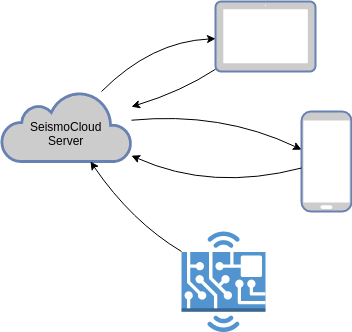
\includegraphics[width=0.5\textwidth]{introduzione/SeismoCloud_arch}
\end{figure}

Dal punto di vista utente, contribuire diventa rapido ed economico: una volta installata la \textit{app}, il sistema si avvia, acquisisce la posizione GPS ed entra a far parte della rete. Si è stimato che, per poter coprire un territorio come quello italiano occorrono dai 3000 ai 4000 sismometri, siano essi \textit{app} per cellulari o dispositivi fisici.

\section{Algoritmo di rilevamento}

\textbf{[inserire immagine del telefono in relazione agli assi cartesiani]}

Il funzionamento del sistema è il seguente: ogni dispositivo (smartphone o dispositivo \textit{IoT}) ha almeno due stati: \textbf{IDLE} e \textbf{QUAKE}. Un dispositivo nello stato di \textbf{IDLE} effettua una rilevazione dell'accelerazione su ogni asse ogni $50ms$, e viene calcolata la componente del vettore risultante mediante la formula~\ref{eq:vettoreris}. Il valore viene quindi confrontato con un valore di soglia calcolato (\ref{eq:soglia}) in modo da filtrare il rumore di fondo e, se la rilevazione risulta superiore alla soglia, il dispositivo informa il server comunicando l'attuale accelerazione rilevata, la posizione geografica ed il momento della rilevazione espresso in tempo UNIX\footnote{Il "tempo UNIX" è definito come il numero di secondi dallo \textit{UNIX Epoch Time}, ovvero dal 1 Gennaio 1970} (con precisione di $\pm1ms$), e successivamene passa allo stato di \textbf{QUAKE}.

\begin{equation} \label{eq:vettoreris}
Acceleration = \sqrt{Value(X)^2 + Value(Y)^2 + Value(Z)^2}
\end{equation}

Per ogni valore rilevato nello stato \textit{IDLE}, inoltre, vengono aggiornati i seguenti valori:
\begin{equation}
\Delta = Acceleration - \rho
\end{equation}
\begin{equation}
\rho = \rho + {\Delta \over |detections|}
\end{equation}
\begin{equation}
\sigma = \sigma + \Delta * (Acceleration - \rho)
\end{equation}
\begin{equation} \label{eq:soglia}
Threshold = \rho + (\sqrt{\sigma \over (|detections|-1)} * \alpha)
\end{equation}

dove: \begin{itemize}
\item $Acceleration \in Z^+$ rappresenta il valore di accelerazione attuale
\item $\rho \in Z^+$ è la media dei valori delle rilevazioni, e $\sigma \in Z^+$ lo scarto quadratico medio, entrambi calcolati mediante un \textit{algoritmo online}\footnote{Un algoritmo viene definito \textit{online} se è in grado di processare un oggetto di input per volta (mantenendo l'invariante che il risultato rappresenta il valore atteso), potenzialmente per un numero infinito di oggetti}
\item $Threshold \in Z^+$ rappresenta la soglia di confronto per il valore di accelerazione, utilizzata per decidere se è da informare il server
\item $\alpha \in Z^+$ rappresenta un valore moltiplicativo fornito dal server (aggiornato a seguito, ad esempio, di eccessive segnalazioni o soglia troppo alta)
\end{itemize}

Il rilevamento, con l'algoritmo sopra citato, avviene in background rispetto all'attività utente: in questo modo si consente il multitasking sul dispositivo e si mantiene l'applicazione sempre attiva in modo trasparente per l'utente.

\chapter{Ottimizzazione energetica: i contesti di attivazione}

Il primo processo di ottimizzazione che è stato portato avanti riguarda i \textbf{contesti di attivazione}. Definiamo il \textbf{contesto di attivazione} come l'insieme delle variabili che rappresentano lo stato del telefono (come: stato batteria, attività utente, etc).

Nella prima versione dell'algoritmo di rilevamento erano presenti solo due stati: \textbf{IDLE} e \textbf{QUAKE}. All'accensione del servizio in background (avviato automaticamente dal sistema all'accensione del telefono), il telefono passava nello stato di \textbf{IDLE} per effettuare le rilevazioni, per poi passare allo stato di \textbf{QUAKE} nel momento di una rilevazione sopra soglia. Chiaramente questo sistema prevedeva che il telefono rimanesse in orizzontale tutto il tempo. Questa prima versione è stata utilizzata in fase di test preliminare per valutare l'efficacia degli algoritmi di soglia e di rilevamento.

Successivamente si è introdotta una prima ottimizzazione: l'attivazione del servizio solo quando il telefono si trova in \textbf{posizione orizzontale} (con le tecniche specificate nel capitolo \ref{chapter:sensori}). Questa seconda versione permette di risparmiare le risorse, ed in particolar modo la batteria (tramite la diminuzione della pressione sulla CPU e memoria), quando il telefono è usato dall'utente oppure non poggiato su una superficie piana (ad esempio, il telefono si trova in una tasca oppure in una borsa). Per stabilire le soglie dei valori da considerare come "rotazione" si è stabilito un \textit{range} di rotazione assoluto rispetto al piano orizzontale, ed un offset di rotazione relativo. \textbf{Questo ci permette di individuare sia il posizionamento non favorevole del telefono, sia una sua rotazione o spostamento in modo repentino}. Quest'ultimo caso è importante perché ci ha permesso di ridurre al minimo i falsi positivi relativi all'azione dell'utente su un cellulare posizionato, fino a quel momento, in orizzontale. Abbiamo quindi introdotto un nuovo stato, lo stato di \textbf{MOVE}. La transizione da uno stato all'altro è determinata dai controlli fatti sui valori dei sensori.

\begin{figure}[ht]
\centering
\label{fig:scs_sm1}
\caption{Diagramma degli stati con Idle, Quake e Move}
\digraph[width=0.8\textwidth]{StateMachine1}{
rankdir=LR;
Quake->Idle [label="Quake motion reported"];
Idle->Quake [label="Quake motion detected"];
Idle->Move  [label="Rotation off-range"];
Move->Idle  [label="Rotation normal"];
}
\end{figure}

Una seconda ottimizzazione è stata apportata dallo spegnimento del servizio per un periodo stabilito quando il telefono si trova in uno stato non utile (\textit{MOVE} ad esempio). E' stato introdotto lo stato di \textbf{MOVE\_BACKOFF}, dove il servizio viene portato dopo un periodo di permanenza in \textit{MOVE}. Questo stato prevede lo \textbf{spegnimento} del servizio, con il rilascio di tutti i WakeLocks\footnote{Un "WakeLock" è un meccanismo di segnalazione, al sistema operativo Android, per la gestione di tutto quello che può impedire o modificare gli stati di risparmio energetico del cellulare, come lo schermo o la CPU principale - se nessuno richiede un WakeLock infatti, il cellulare va in uno stato di quiete per cui la CPU principale, il WiFi e altri chip vengono spenti}. Per decidere quando riattivare il servizio (e controllare se ci sono le condizioni per passare allo stato di \textit{IDLE}) viene utilizzato un algoritmo di \textit{backoff esponenziale}: al primo passaggio allo stato di \textbf{MOVE\_BACKOFF} il tempo per il risveglio (e quindi il prossimo controllo) viene impostato a 30 secondi. Successivamente, se il controllo fallisce (quindi rimaniamo dentro \textbf{MOVE}) il tempo viene raddoppiato ogni volta, fino ad un massimo di 900 secondi.

In questo modo il servizio, durante il periodo di \textbf{MOVE\_BACKOFF}, non consuma risorse e non detiene nessun tipo di WakeLock, permettendo quindi al telefono di andare in \textit{stand-by} e gestire il sistema come se SeismoCloud non fosse installato. Il consumo determinato dalla nostra app, quindi, mentre il telefono è in uso oppure in posizione non orizzontale è zero. Il risveglio invece è gestito dal sistema operativo \textbf{Android}, il quale gestisce in modo ottimizzato gli interrupt basati sul tempo (come questo per la riattivazione del servizio), spesso (sui telefoni che lo supportano) con un chip dedicato a consumo molto ridotto.

\begin{figure}[ht]
\centering
\label{fig:scs_sm2}
\caption{Diagramma degli stati con Idle, Quake, Move e Move\_Backoff}
\digraph[width=\textwidth]{StateMachine2}{
rankdir=LR;
Quake->Idle [label="Quake motion reported"];
Idle->Quake [label="Quake motion detected"];
Idle->Move  [label="Rotation off-range"];
Move->Idle  [label="Rotation normal"];
Move_Backoff->Move  [label="Interrupt (timeout)"];
Move->Move_Backoff  [label="Persistent Move state"];
}
\end{figure}

Una ulteriore ottimizzazione è stata l'introduzione del controllo sulla effettiva disponibilità del segnale GPS: sia in fase iniziale (quello che, nel lessico del \textit{Global Position System} viene definito come \textit{fix-iniziale}) sia durante il funzionamento (stato \textbf{IDLE}), il sistema controlla l'effettiva presenza del segnale GPS per la localizzazione. Questo permette di individuare diversi comportamenti:

\begin{itemize}
\item \textbf{Disattivazione del sensore GPS} da parte dell'utente (tramite apposita opzione di Android) oppure perdita del segnale
\item \textbf{Spostamento} del telefono (data la precisione del GPS, spostamento in termini di \textit{metri})
\end{itemize}

In entrambi i casi il servizio non è più in grado di fare affidamento alla posizione memorizzata, dunque entra nello stato di \textbf{MOVE\_BACKOFF}, dove continuerà ad essere fino al ritorno del segnale GPS (nel primo caso) o ad una posizione fissa (nel secondo caso). Questo ha permesso di ridurre, come da test effettuati, il consumo di batteria in particolari condizioni: ad esempio posizionare il telefono sul cruscotto di una automobile, o su di un tavolino del treno, avrebbe comportato l'attivazione del servizio a causa della posizione orizzontale. Tuttavia, i dati di accelerazione sarebbero stati ovviamente inutili, ai fini dell'indentificazione del terremoto. Dunque, \textbf{con questa nuova aggiunta il sistema è in grado di rilevare questi casi} e si pone nello stato corretto.

Ulteriore riduzione del consumo è stata fatta considerando un altro fattore importante per i sistemi \textit{IoT}, ovvero la presenza della connessione di rete (Wi-Fi o rete cellulare). Qualora venga a mancare la connessione di rete, di nuovo il sistema è portato nella posizione di \textbf{MOVE\_BACKOFF} con l'algoritmo sopra citato. Questo permette di risparmiare batteria nei luoghi dove e nei momenti quando il segnale è assente.

Infine, è stata fatta una analisi sulla batteria e sul consumo. In prima istanza è stato considerato lo status di "\textbf{risparmio energia}" che Android attiva nel momento in cui la batteria raggiunge un valore prefissato (in genere, a meno di cambiamenti fatti dall'utente, il valore è il 15\% della capacità). Grazie ad un \textit{handler} viene intercettato questo evento e viene posto il servizio nella fase di \textbf{MOVE\_BACKOFF} indipendentemente dalle condizioni favorevoli sopra citate. Dopodiché si è provveduto ad effettuare uno studio approfondito, con diversi test, meglio specificata nel capitolo \ref{chapter:batteria}.

Infine quindi, il nostro \textbf{contesto di attivazione} si compone delle variabili:

\begin{itemize}
\item Rotazione/posizione favorevole o no alla lettura del dato
\item Persistenza della posizione sfavorevole nel tempo
\item Presenza o meno della localizzazione GPS
\item Presenza o meno di uno spostamento geografico
\item Presenza o meno della rete Internet
\item Status di risparmio energetico del sistema operativo (capacità batteria rimanente)
\end{itemize}

Un contesto di attivazione non corretto non permette al servizio di ripartire, e quindi di consumare batteria, CPU e memoria. Il diagramma a stati:

\begin{figure}[ht]
\centering
\label{fig:scs_sm3}
\caption{Diagramma degli stati finale}
\digraph[width=\textwidth]{StateMachine3}{
rankdir=LR;
Quake->Idle [label="Quake motion reported"];
Idle->Quake [label="Quake motion detected"];
Idle->Move  [label="Rotation off-range"];
Move->Idle  [label="Rotation normal"];
Move_Backoff->Move  [label="Interrupt (timeout)"];
Move->Move_Backoff  [label="Persistent Move state"];
Idle->Move_Backoff  [label="Location unavailable/move"];
Idle->Move_Backoff  [label="Android Power safe mode"];
Idle->Move_Backoff  [label="Internet unavailable"];
}
\end{figure}

Il diagramma degli stati completo è rappresentato nel workflow del servizio, rappresentato dalla figura \ref{fig:serviceflowdiagram} a pagina \pageref{fig:serviceflowdiagram}.

\chapter{Ottimizzazione energetica: i sensori}
\label{chapter:sensori}

Si spiega anche l'attivazione programmata del magnetometro dopo l'attività dell'accelerometro, inizialmente pensata per risparmiare CPU ed energia, e come questo meccanismo sia stato dismesso poiché effettivamente non comportava nessun risparmio energetico (il sistema mag+accel è sempre attivo).

\chapter{Ottimizzazione energetica: la curva di scarica}
\label{chapter:batteria}

Qui parlo dell'algoritmo che segue la curva di scarica. Tips: mostrare i dati provenienti dal database con interrogazioni statistiche

\chapter{Ottimizzazione del processore: la comunicazione con il front-end}

Qui si descrive la politica utilizzata per mantere l'applicazione attiva (notifica permanente) poiché Android pone le applicazioni in sleep. Si spiega anche il wakelock sulla CPU, la sospensione dell'aggiornamento dati in background delle activity quando non sono in vista.

\chapter{Ottimizzazione della rete: MQTT}

Si spiega come l'introduzione dell'MQTT abbia ridotto il carico sulla rete per lo scambio dati con il server.

\chapter{Ottimizzazione della rete: Pushback}

Parlare del meccanismo di Pushback per l'invio dei dati (ad esempio survey) in background in modo ottimizzato in caso di problemi di rete (invio asincrono).

\chapter{Ottimizzazione dell'uso di memoria nel codice}

Qui si descrive la politica utilizzata, nella costruzione del codice, per minimizzare lo spreco di memoria (esempio: media/varianza mobile).

\pagebreak

\begin{figure}[ht]
\centering
\label{fig:serviceflowdiagram}
\caption{Diagramma di flusso del servizio SeismoCloud}
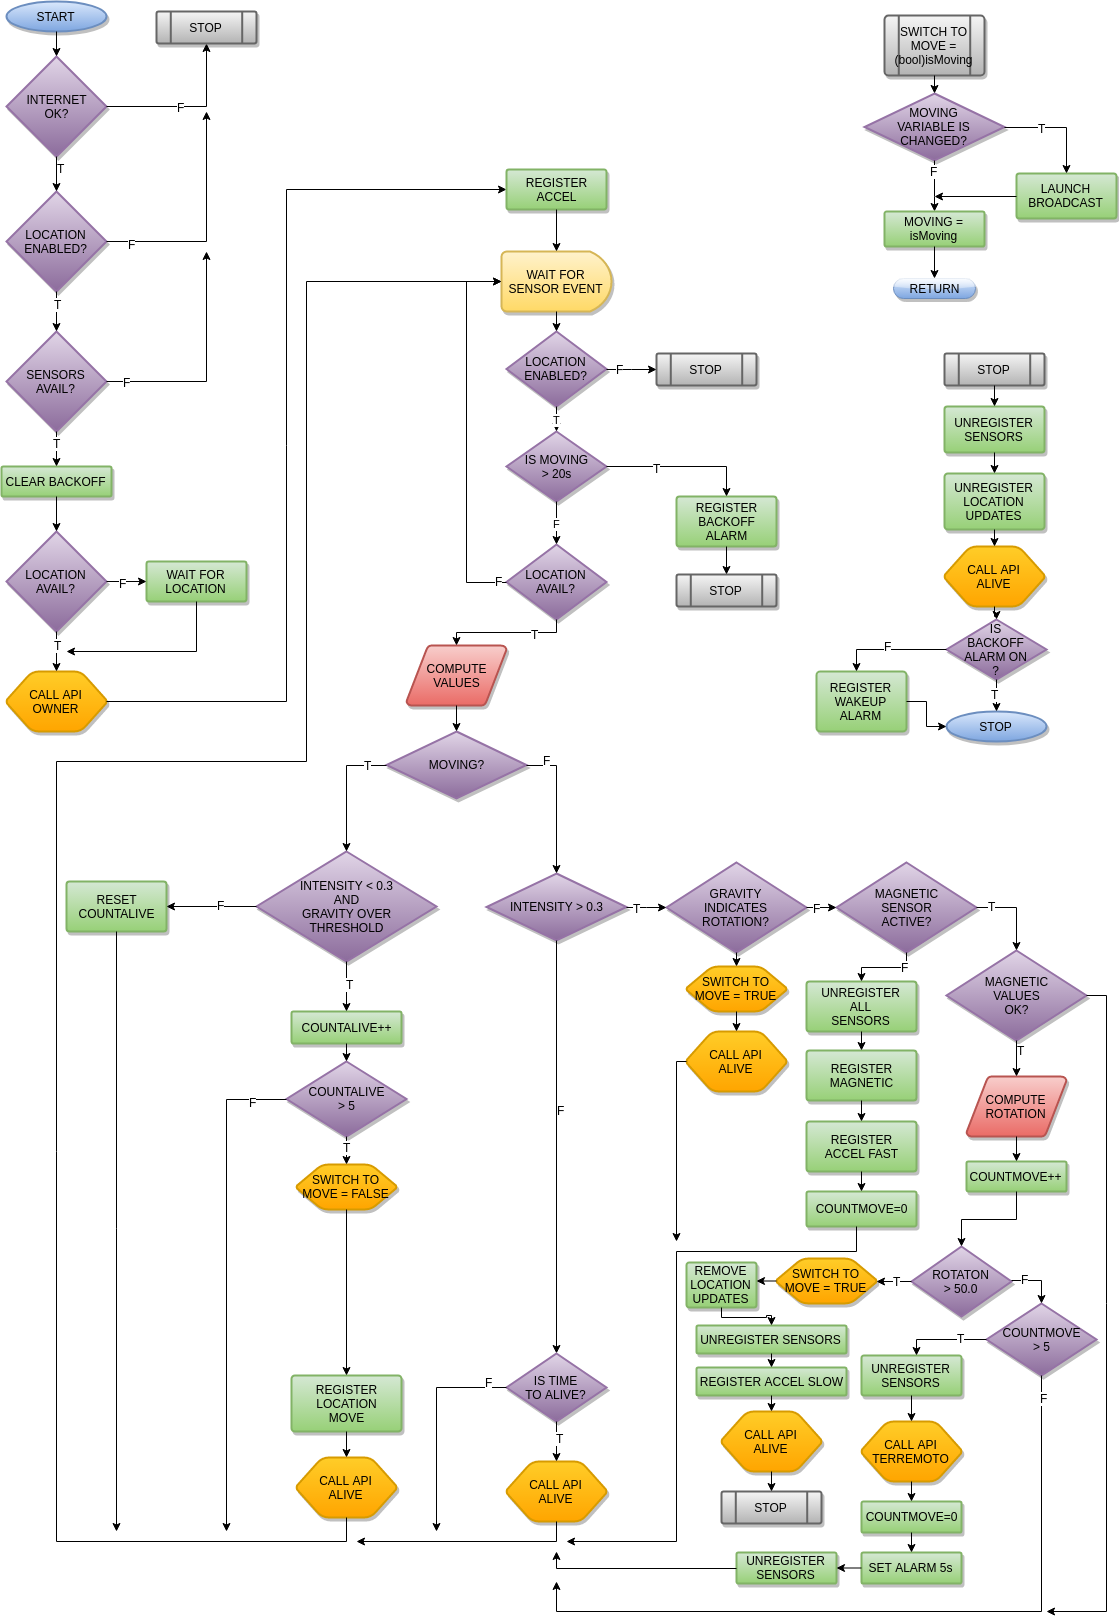
\includegraphics[width=\textwidth]{introduzione/SeismoCloud_flowdiag}
\end{figure}

%
%\chapter{Sviluppo e test}
%
%Si spiega l'adozione di particolari meccanismi per la gestione ottimizzata del processo di sviluppo:
%
%\begin{itemize}
%\item Utilizzo della libreria ACRA per l'immediata segnalazione di errori della app (da produzione)
%\item Utilizzo della libreria LeakCanary per la ricerca di memory leak
%\item Utilizzo delle librerie Parceler e Android Annotations per ridurre la quantità di codice ridondante
%\item Sistemi di controllo versione: branch per funzionalità, sviluppo parallelo
%\item Continuos integration per la verifica dei build ed instrumentation test
%\item Verifica del codice tramite SonarQube per aderenza agli standard Java/Android e risultati di analisi statica del codice
%\end{itemize}

\chapter{Sviluppi futuri}

\begin{itemize}
\item Utilizzo di un sistema di spegnimento controllato dal server per l'ottimizzazione geografica
\item Utilizzo di sensori dedicati (es. Samsung Significant Motion Sensor) per il wake-up
\item Riscrittura parti critiche in codice nativo per l'esecuzione ottimizzata e rapida (con conseguente aumento del periodo di idle del telefono)
\end{itemize}

\end{document}
